\documentclass[tikz]{standalone}

\usepackage[utf8]{inputenc}
\usepackage[T1]{fontenc}
\usepackage{cmap}
\usepackage{amsmath}
\usepackage{amssymb}
\usepackage{verbatim}
\usepackage{bm}

\renewcommand{\familydefault}{\sfdefault}
\usepackage[cm]{sfmath}

\usetikzlibrary{bending}
\usetikzlibrary{decorations.pathreplacing}
\usetikzlibrary{decorations.pathmorphing}
\usetikzlibrary{fadings}
\usetikzlibrary{shapes}

\definecolor{cblue}{rgb}{0.122, 0.467, 0.706}
\definecolor{corange}{rgb}{1, 0.498, 0.055}
\colorlet{lightgray}{black!20}

\begin{document}
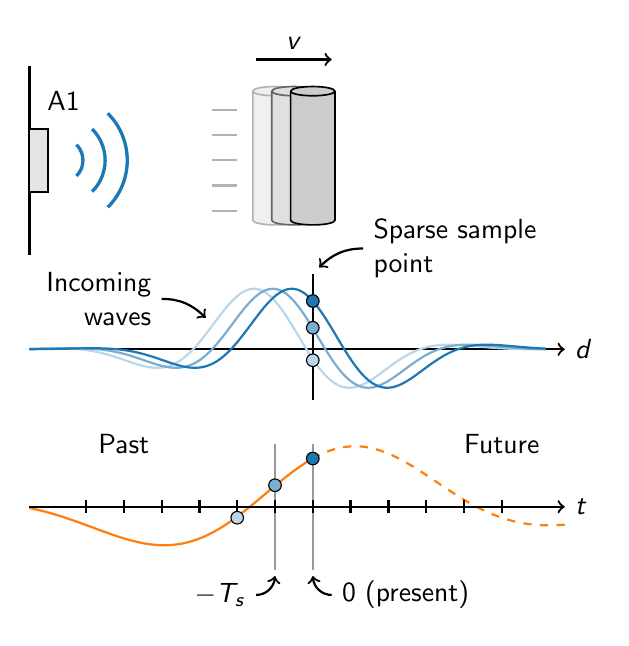
\begin{tikzpicture}[scale=0.8]

\draw [very thick] (0, 0) -- (0, -3);
\draw [fill=black!10, thick] (0, -1) rectangle ++(0.3, -1);
\draw [cblue, very thick, decoration=expanding waves, segment length=8pt, decorate] (0.5, -1.5) -- ++(1.2, 0);
\node [above right=3pt] at (0, -1) {A1};

\foreach \x/\inten in {-2/30, -1/60, 0/100}
    \node [color=black!\inten, fill=lightgray!\inten, semithick, cylinder, shape border rotate=90, draw, aspect=0.5, minimum height=50pt, minimum width=16pt]
        at (4.5 + \x * 0.3, -1.5) {};

\draw [thick, ->] (3.6, 0.1) -- node [above] {$v$} (4.8, 0.1);

\foreach \y in {-2, ..., 2}
    \draw [thick, black!30] (2.9, -1.5+0.4*\y) -- ++(0.4, 0);

\draw [thick] (4.5, -3.3) -- ++(0, -2.0);
\draw [thick, ->] (0, -4.5) -- ++(8.5, 0) node[right]{$d$};

\draw [thick, <-] (4.5, -3.3) ++(0.1, 0.1) to [out=45, in=180] ++(0.7, 0.3) node[right, text width=70pt]{Sparse sample point};

\foreach \xshift/\inten in {-0.6/30, -0.3/60, 0/100} {
    \draw [cblue!\inten, thick, domain=-4.5:3.7, smooth, samples=200, variable=\x, shift={(4.5, -4.5)}]
        plot ({\x}, {exp(-(\x-\xshift)*(\x-\xshift)*0.3) * sin(100*(\x-\xshift)+130)});

    \draw [fill=cblue!\inten] (4.5, {sin(100*(-\xshift) + 130) - 4.5}) circle (1mm);
}

\draw [thick, <-] (2.8, -4) to [out=135, in=0] ++(-0.7, 0.3) node [left, text width=40pt, align=right] {Incoming\\waves};

\draw [corange, thick, domain=0:4.5, smooth, samples=200, variable=\x, shift={(4.5, -7)}]
        plot ({-\x}, {exp(-\x/2*\x/2*0.3) * sin(100*(\x/2) + 130)});

\draw [corange, dashed, thick, domain=-4:0, smooth, samples=200, variable=\x, shift={(4.5, -7)}]
    plot ({-\x}, {exp(-\x/2*\x/2*0.3) * sin(100*(\x/2) + 130)});


\draw [thick, black!40] (4.5, -6) -- ++(0, -2.0);
\draw [thick, <-] (4.5, -8)++(0, -0.1) to [out=270, in=180] ++(0.3, -0.3) node[black, right]{$0$ (present)};

\draw [thick, black!40] (4.5-0.6, -6) -- ++(0, -2.0);
\draw [thick, <-] (4.5-0.6, -8)++(0, -0.1) to [out=270, in=0] ++(-0.3, -0.3) node[black, left]{$-T_s$};

\draw [thick, ->] (0, -7) -- ++(8.5, 0) node[right]{$t$};

\foreach \x in {-6, ..., 5}
    \draw [thick] ({\x*0.6+4.5}, -7) ++(0, 0.1) -- ++(0, -0.2);

\node at (4.5-3, -6) {Past};
\node at (4.5+3, -6) {Future};

\foreach \xshift/\inten in {-0.6/30, -0.3/60, 0/100} {
    \draw [fill=cblue!\inten] ({4.5 + \xshift * 2}, {sin(100*(-\xshift) + 130) - 7}) circle (1mm);
}

\end{tikzpicture}
\end{document}
